\documentclass[border=6pt]{standalone}
\usepackage{tikz}
\begin{document}
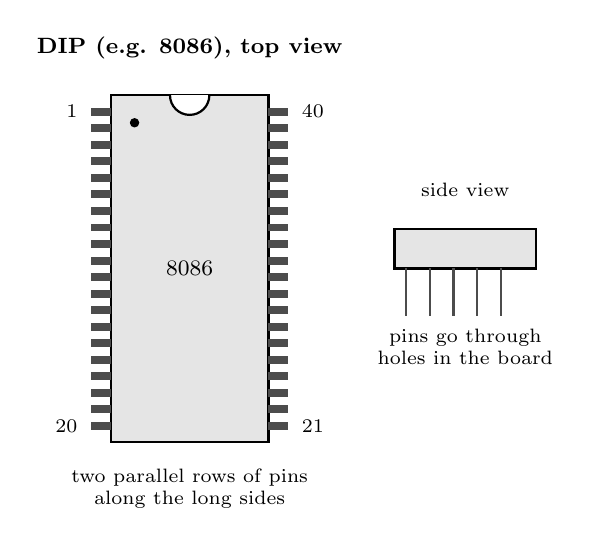
\begin{tikzpicture}[font=\small]
% DIP top view
\node[font=\footnotesize\bfseries] at (1.0,5.0) {DIP (e.g. 8086), top view};
\draw[thick,fill=gray!20] (0,0) rectangle (2.0,4.4);
\draw[thick,fill=white] (0.75,4.4) arc[start angle=180,end angle=360,radius=0.25];
\fill (0.3,4.05) circle (0.06);
\node[font=\footnotesize] at (1.0,2.2) {8086};
\foreach \i in {1,...,20} {
  \pgfmathsetmacro{\y}{4.4-0.21*\i}
  \fill[gray!60!black] (-0.25,\y-0.05) rectangle (0,\y+0.05);
  \fill[gray!60!black] (2.0,\y-0.05) rectangle (2.25,\y+0.05);
}
\node[font=\scriptsize,anchor=east] at (-0.3,4.19) {1};
\node[font=\scriptsize,anchor=east] at (-0.3,0.2) {20};
\node[font=\scriptsize,anchor=west] at (2.3,0.2) {21};
\node[font=\scriptsize,anchor=west] at (2.3,4.19) {40};
\node[font=\scriptsize,align=center] at (1.0,-0.6) {two parallel rows of pins\\along the long sides};
% side view of DIP
\begin{scope}[xshift=3.6cm,yshift=1.6cm]
\node[font=\scriptsize] at (0.9,1.6) {side view};
\draw[thick,fill=gray!20] (0,0.6) rectangle (1.8,1.1);
\foreach \x in {0.15,0.45,...,1.65} \draw[thick,gray!60!black] (\x,0.6) -- (\x,0);
\node[font=\scriptsize,align=center] at (0.9,-0.4) {pins go through\\holes in the board};
\end{scope}
\end{tikzpicture}
\end{document}
